\chapter{Constructing Compact Causal Mathematical Models for Complex Dynamics}
\label{cha:ch2}
The behavior of complex systems is influenced over many \textit{space} and \textit{time scales} by multi-physics interactions. From cellular interactions within the microbiome-to-brain architecture, to organ interdependencies within human body expressed via signature physiological processes, to animal swarms and food webs, to social groups and society, \textbf{memory}, \textbf{interdependency} and \textbf{concurrency} are fundamental characteristics. Although recent advances in sensing technology contributed to large datasets, the modeling and analysis of complex systems have mainly focused on modeling frameworks that ignore the exhibited long-range memory, spatio-temporal fractality, non-linear, non-ergodic and non-Gaussian properties. More precisely, traditional mathematical modeling approaches in nonlinear dynamical systems, statistical machine learning, statistical signal processing and process control, system identification and econometrics focussed on describing the complex system dynamics via a set of integer-order ordinary differential equations (ODEs) (see eq. (\ref{nonlinearODE})) and identify the parameters of the model by minimizing a cost function that depends on a goodness-of-fit metric (i.e., the difference between the data and the postulated model class) and a complexity of the model penalty metric \cite{Ljung2010}:
\begin{eqnarray}
\label{nonlinearODE}
&\frac{\displaystyle dx_{j}(t)}{dt} = f_{j}(x_{1},...,x_{n},u_{1},...,u_{m},\theta_{j})&
\end{eqnarray} 
where the function $f_{j}$ encodes the linear/nonlinear interdependencies between the state variables $x_{1},...,x_{n}$ and the control variables $u_{1},...,u_{m}$, and $\theta_{j}$ represents the set of parameters to be estimated from measured time series. 

For instance, with the aim of determining equations of motion from observations of time-dependent behavior, Crutchfield and McNamara  developed an informational measure to quantify the modeling accuracy for eq. (\ref{nonlinearODE}) from time series observations and identifies the parameters of the ODEs by minimizing the distance between the data and the postulated model \cite{crutchfield1987}. Relying on the assumption that the observed dynamical system is memoryless (i.e., the rate of change of its state variables obeys an integer order time derivative), the heuristic modeling strategy proposed in \cite{Packard1980} first constructs a phase-space plot from the observations of a single variable (ignoring the true causal interdependency) and determines the dimensionality of the system's attractor. Building on postulating a particular integer order time derivative coupled with a specific nonlinear mathematical expression and using the Ritt's algorithm of differential algebra, one can find the parameters of the model by solving a regression problem \cite{Ljung1994global}. Using a bilinear approximation of the dynamics of interactions between system variables, the dynamic causal modeling in \cite{Friston2003} proposes a Bayesian framework that determines the parameters of a multi-dimensional linear (integer order) dynamical system (the dynamics is assumed to be memoryless). Along the same lines, numerous other approaches (e.g., manifold learning \cite{Ohlsson2008}, Bayesian networks \cite{Chiuso2016}, Q-learning~{\cite{mehta2009q}}, variational inference \cite{Opper2008}) have been proposed in the literature. More recently, a kernel cross-spectral density based analysis of stationary time series was proposed for measuring the independence and the similarity between various time series \cite{Besserve2013}. 

While not being able to be exhaustive in covering all previous work, the implicit assumption in all these prior approaches is that the \textit{dynamics is intrinsically governed by a first order time derivative which implies that the inter-event times between successive changes in the magnitude of the processes are characterized by an exponential law}. However, many complex systems exhibit \textbf{long-range memory}~\cite{svenkeson2016spectral} and \textbf{fractal dynamics} that are characterized by power (non-exponential) law magnitude and inter-event times bringing into question whether the nonlinearity should be considered in the time or space domains or both~\cite{shlesinger1993strange,bassingthwaighte1994properties,west2012fractal,bogdan2015mathematical}.  

In addition, a number of outstanding challenges remain for constructing mathematical models of complex systems: (\textit{i}) How can we distinguish between spatial and temporal nonlinearity and how can we construct mathematical models (i.e., dynamical equations) that capture the spatio-temporal statistical characteristics of complex systems? (\textit{ii}) How can we identify the mathematical expressions of the functions $f_{j}$ for the nonlinear models of complex systems and determine the degree of nonlinearity that should be accounted for without incorporating unnecessarily many nonlinear terms? (\textit{iii}) How can the power law and non-Gaussian properties of the magnitudes observed in many time series impact the degree of nonlinearity? (\textit{iii}) How one can interpret the asymmetry observed in the time series realization of various processes and estimate the amount of information gained from analyzing the spatio-temporal complexity present in time series?

 To overcome the afore-mentioned drawbacks, in this paper, we seek to understand mathematically how various fundamental and essential components of the complex systems interact and exchange information to influence the overall performance and behavior. To the best of our knowledge, this paper is the first to investigate the impact of microscopic dynamics encapsulated in the ordered sequence of magnitude increments and inter-event times of the stochastic process. More precisely, \textbf{we have made the following novel contributions in this work}:
 
 \textbf{Firstly}, we show that by adopting a causal inference like framework and combining with probabilistic tools that were originally developed in statistical physics context we can develop mathematical strategies that can enable us to distinguish when a time series exhibits a short-range or a long-range dependence dynamics. 
 
 \textbf{Secondly}, we show how the analysis of a multi-point probability density function can be interpreted through the lens of maximum entropy principle and distinguish between a memoryless or a complex time-dependency structure. 
 
 \textbf{Thirdly}, this analysis allows to identify conditions under which a complex system under investigation can be approximated through a single order (i.e., the inter-event times can be characterized by a marginal power law distribution being reminiscent of mono-fractal dynamics) or multiple order (i.e., the inter-event times and overall system dynamics requires multiple interwoven power laws and multiple scaling exponents being reminiscent of multi-fractal dynamics) fractional dynamics.
\begin{figure}%[!htb]
\centering
\includegraphics[width=1\columnwidth]{overview.eps}
\caption{\textbf{The overview of the proposed framework to construct compact mathematical modeling of complex dynamics and its application to the development of closed-loop cyber-physical systems. The monitored physical process is interfaced with a data-driven learning framework that investigates the system dynamics from a microscopic perspective (e.g., magnitude and inter-event time increments). A non-Markovian probabilistic description is constructed based on generalized master equation and the principle of maximum causal entropy to encapsulate the exhibited power-law behaviors (Section 2.1 and Section 2.2). This master equation based formalism allows the derivation of the nonlinear dynamical state equations with minimal postulation to capture system dynamics (Section 2.3). By retrieving the system model parameters from a specific physical process from which the model is derived, the proposed framework can serve as the intelligent core of the closed-loop intelligent cyber-physical systems for a wide spectrum of CPS applications( e.g., decode the neuron activities to generate stimulation signals for the control of prothesis or muscles to help amputee or paralyzed patients to regain body functionality).}}
\label{fig:overview}
\vskip -1mm
\end{figure} 
  With respect to the afore-mentioned question (\textit{i}), the proposed mathematical formalism allows us to determine when the space and time components of a stochastic process can be decoupled and its overall evolution be described through a multi-fractional nonlinear partial differential equation (PDE) for the probability to reach a state at a particular point in time. 
  
  With respect to the afore-mentioned question (\textit{ii}), we demonstrate how the power law behavior exhibited in the space (magnitudes) and time (intervals of time between successive changes in the magnitude) domains can be encapsulated through a compact fractional calculus representation for the  probability to reach a state at a particular point in time and how this new formalism enables the derivation of the nonlinear dynamical equations with minimal postulation. Simply speaking, the statistical analysis of the magnitudes and the inter-event times dictates the mathematical expression (form) of the dynamical model. 
  
  With respect to the afore-mentioned question (\textit{iii}), we illustrate how the asymmetry observed between the positive and negative increments in the magnitude of the stochastic process can be encoded through Riesz-Feller fractional order operators leading to a new class of multi-fractional nonlinear PDEs that could be exploited for computing information theoretic metrics regarding the modeling accuracy and overfitting. This is left for future work. 
%\section{Related Work and Novel Contribution}
%\label{s:RelatedWork}
\section{Compact Mathematical Modeling of Complex Dynamics}
\label{s:MathematicalModeling}
We show in Figure~\ref{fig:overview} the overview of the proposed framework that enables the construction of the compact mathematical causal modeling of the complex dynamics in a wide spectrum of applications in cyber-physical domain. By setting up sensors that monitor the physical process of interest, we are able to investigate the microscopic dynamics of the underlying system evolution in both space (magnitude increments) and time (inter-event times). We demonstrate that the interdependency between the jumps of the magnitude and inter-event times i) dictate the mathematical characterization of changing rate of system states and ii) impact the degree of nonlinearity of the couplings among system components. To capture these properties, we propose a non-Markovian probabilistic description of the physical process through generalized master equation. By principle of maximum causal entropy considering the power-law behavior exhibited in the system dynamics, we are able to derive the nonlinear dynamical state equations with minimal postulation. 

By leveraging the system identification techniques to retrieve the model derived by learning the microscopic dynamics of the observed physical process, the proposed causal modeling of complex dynamics can be integrated as the core of the intelligent cyber-physical systems in a widely ranged CPS applications such as the prediction of system dynamic behaviors, the detection of system anomalies and the synthesis of the closed-loop controllers for autonomous systems. In what follows, we will present the detailed discussion on all components of our proposed mathematical modeling framework.

\subsection{Microscopic Dynamics Dictates the Governing Mathematical Equation}
\label{s:Microscopic}
We consider a stochastic process $x(t)$, whose realization is described by a tuple sequence of magnitude and time increments: $ \{ (\Delta x_{1},\Delta t_{1});$ $ (\Delta x_{2},\Delta t_{2});\ldots ; (\Delta x_{m},\Delta t_{m}) \}$ (see Figure 1). More precisely, the $\Delta t_{j}$ represents the waiting time in which the stochastic process makes a jump $\Delta x_{j}$ in the $j$-th iteration. To define the underlying stochastic process (sequence), we introduce the conditional probability density function 
\begin{eqnarray}
w(\Delta x_{m},\Delta t_{m}|\Delta x_{m-1},\Delta t_{m-1}\ldots;\Delta x_{1},\Delta t_{1}) =  \nonumber\\
= w(\Delta x_{m},\Delta t_{m}|\Delta x_{1:m-1},\Delta t_{1:m-1})
\end{eqnarray}
%the causally conditional probability density function:
%\begin{eqnarray}
%w(\Delta x_{1:m}||\Delta t_{1:m}) = \prod\limits_{j=1}^{m} w(\Delta x_{j} | \Delta x_{1:j-1}, \Delta t_{1:j})
% \end{eqnarray}
and the joint probability density function (PDF):
\begin{eqnarray}
w(\Delta x_{m},\Delta t_{m};\ldots;\Delta x_{1},\Delta t_{1}) =  w(\Delta x_{1:m},\Delta t_{1:m}) =\nonumber\\
=  \prod\limits_{j=1}^{m} w(\Delta t_{j}|\Delta t_{1:j-1})\prod\limits_{j=1}^{m}w(\Delta x_{j}|\Delta x_{1:j-1},\Delta t_{1:m})
\end{eqnarray}
where we have taken into account the chain rule and the causal dependency. The rationale for considering these probabilities is motivated by the need to understand how the so called microscopic dynamics influences the overall evolution; alternatively stated we aim to understand: \textit{i}) How the changes in the magnitude increments affect the degree of linearity /nonlinearity of the function $f_{j}$ in equation (\ref{nonlinearODE}); \textit{ii}) How the statistics of the inter-event times impact the overall dynamics and could dictate the mathematical operator characterizing the rate of change in the system. 

%Using concepts from the Marko-Massey theory of directed information \cite{}\cite{}, the joint PDF $w(\Delta x_{1:m},\Delta t_{1:m})$ can be expressed in terms of causal conditional PDFs as follows:
%\begin{eqnarray}
%w(\Delta x_{1:m},\Delta t_{1:m}) = w(\Delta x_{1:m} || \Delta t_{1:m-1}) w(\Delta t_{1:m} || \Delta x_{1:m})
%\end{eqnarray}

 One fundamental assumption we make is that the tuple $(\Delta x_{j}, \Delta t_{j})$ is not random and independent of the previous magnitude increments $(\Delta x_{i}, \Delta t_{i})$ with $ 1 \leq i < j$. Instead, we assume that the ordered sequence $ \{ (\Delta x_{1},\Delta t_{1}); (\Delta x_{2},\Delta t_{2}); \ldots ; (\Delta x_{m},\Delta t_{m}) \}$ posses some form of directed information that is conveyed either from the space of magnitudes $\Delta x_{j}$ to that of time increments $\Delta t_{j}$ or from the space of time increments  $\Delta t_{j}$ to that of the process magnitudes  $\Delta x_{j}$ from one iteration (generation) to another (preserving the axis of time). This ordered dependency represents the source of the fractal behavior that could be observed in either the magnitudes or the waiting (inter-event) times. Consequently, in this work, we investigate how this directional information and its related statistics determine the type of dynamical equation that governs the evolution of process $x(t)$. An important problem in establishing a governing dynamical state equation (i.e., a differential equation describing the evolution of the $k$-th order statistical moments) is represented by the need to elucidate the dependency structure between the process magnitudes and time increments and the mathematical form of the joint PDF $w(\Delta x_{m},\Delta t_{m};\ldots;\Delta x_{1},\Delta t_{1})$.  
 
 In order to describe a strategy for investigating the dependency structure between the process magnitudes and time increments, we assume that the stochastic process $x(t)$ corresponds to a non-extensive\footnote{Systems obey non-extensive statistical mechanics where entropy is non-additive} system and introduce the following definitions:

\textit{Definition 1:} (\cite{Tsallis1987}) Given a continuous probability distribution $f(x,y)$, the non-extensive Tsallis entropy is defined by:
\begin{eqnarray}
S_{q}[f] = \frac{1}{q-1}\int\limits_{x_{min}}^{x_{max}}\int\limits_{y_{min}}^{y_{max}}\{ f(x,y) - f(x,y)^{q}\}dxdy
\end{eqnarray} 
where $q$ is a real number and represents the entropic index. When $q \rightarrow 1$ the above formula reduces to the Boltzmann-Gibbs or Shannon entropy (up to a constant parameter).

\textit{Definition 2:} Given two continuous joint probability distributions $w(\Delta x_{1:m}, \Delta t_{1:m})$ and $w(\Delta x_{1:m-1}, \Delta t_{1:m-1})$, we define the causal non-extensive Tsallis entropy as follows:
\begin{eqnarray}
S_{q}(\Delta x_{m}, \Delta t_{m}|\Delta x_{1:m-1}, \Delta t_{1:m-1}) = \frac{1}{q-1} \int \ldots \int \nonumber\\
\{ \frac{w(\Delta x_{1:m},\Delta t_{1:m})}{w(\Delta x_{1:m-1},\Delta t_{1:m-1})}[\frac{w(\Delta x_{1:m},\Delta t_{1:m})^{1-q} }{w(\Delta x_{1:m-1},\Delta t_{1:m-1})^{1-q} }- 1] \} 
\end{eqnarray}

%\textit{Definition 2:} The cumulative causal nonextensive Tsallis entropy of $\Delta x_{m}$ and $\Delta t_{m}$ given $\Delta x_{1:m-1}$ and $\Delta t_{1:m-1}$ is
%\begin{eqnarray}
%S_{q} (\Delta x_{m}, \Delta t_{m} ||| \Delta x_{1:m-1}, \Delta t_{1:m-1}) =   \int d(\Delta x_{m})  \nonumber\\
% \int d(\Delta t_{m}) \ldots \int d(\Delta x_{1}) \int d(\Delta t_{1})  \frac{w(\Delta x_{1:m},\Delta t_{1:m})}{q-1}\nonumber \\
% \{ \prod\limits_{j=1}^{m} w(\Delta x_{j}, \Delta t_{j}| \Delta x_{1:j-1},\Delta t_{1:j-1})^{1-q} - 1 \} = \nonumber\\
% =  \int ... \int \{ \frac{w(\Delta x_{1:m},\Delta t_{1:m})}{q-1} \frac{w(\Delta x_{1:m},\Delta t_{1:m})^{1-q}}{w(\Delta x_{1},\Delta t_{1})^{1-q}} \nonumber \\
%  - \frac{w(\Delta x_{1:m},\Delta t_{1:m})}{q-1} \} d(\Delta x_{m}) ... d(\Delta t_{1})
% \end{eqnarray}

%\textit{Definition 4:} The partial causal nonextensive Tsallis entropy of $\Delta x_{m}$ and $\Delta t_{m}$ given $\Delta x_{1:m-1}$ and $\Delta t_{1:m-1}$ is
%\begin{eqnarray}
%&S_{q} (\Delta x_{m}, \Delta t_{m} ||| \Delta x_{1:m-1}, \Delta t_{1:m-1}) =   \frac{1}{q-1}  \int d(\Delta x_{m})  &\nonumber\\
%&\int d(\Delta t_{m}) \ldots \int d(\Delta x_{1}) \int d(\Delta t_{1})  w(\Delta x_{1:m},\Delta t_{1:m}) &\nonumber \\
% &\{ \prod\limits_{j=1}^{m} w(\Delta x_{j}, \Delta t_{j}| \Delta x_{1:j-1},\Delta t_{1:j-1})^{1-q} - 1 \} = & \nonumber\\
% &= \int ...\int \{ \frac{w(\Delta x_{1:m},\Delta t_{1:m})}{q-1} \frac{w(\Delta x_{1:m},\Delta t_{1:m})^{1-q}}{w(\Delta x_{1},\Delta t_{1})^{1-q}} & \nonumber \\
%  & - \frac{w(\Delta x_{1:m},\Delta t_{1:m})}{q-1} \} d(\Delta x_{m}) ... d(\Delta t_{1}) &
% \end{eqnarray}

As will be shown in the next subsection, the mathematical expression of the joint PDF $w(\Delta x_{1:m},\Delta t_{1:m})$ plays a crucial role in establishing the dynamical equations of the $k$-th order statistical moments. Consequently, in order to elucidate the form of the joint PDF $w(\Delta x_{1:m},\Delta t_{1:m})$ we employ the principle of maximum entropy which describes a probability distribution estimator that best represents the state of knowledge or known properties of that distribution~\cite{montroll1983maximum}. Simply speaking, this estimator implies maximizing an entropic functional subject to constraints that reflect our knowledge about the distribution (e.g., normalization condition, fractional order statistical moments). In what follows, we will describe a maximum entropy inspired estimator for the joint PDF $w(\Delta x_{1:m},\Delta t_{1:m})$ and its related probabilistic components.

\textit{Definition 3:} The \textit{principle of maximum causal non-extensive entropy} describes the causal non-extensive entropy-maximizing probability distribution estimator, $\hat{w}(\Delta x_{m},\Delta t_{m}|\Delta x_{1:m-1}, \Delta t_{1:m-1})$, by solving the following optimization problem: 
\begin{eqnarray}
\label{PrincipleOfMaximumPartialConditionalEntropy}
&max_{\hat{w}(\Delta x_{1:m},\Delta t_{1:m})}  \{ S_{q}[\hat{w}(\Delta x_{1:m-1},\Delta t_{1:m-1})] + &\nonumber \\
&S_{q}(\Delta x_{m}, \Delta t_{m}| \Delta x_{1:m-1}, \Delta t_{1:m-1}) \} &\\
&\int \ldots \int \hat{w}(\Delta x_{1:m},\Delta t_{1:m}) d(\Delta x_{m}) \ldots d(\Delta t_{1}) = 1 &  \\
&\int ... \int \hat{w}(\Delta x_{1:m-1},\Delta t_{1:m-1}) d(\Delta x_{m-1}) ... d(\Delta t_{1}) = 1 &  \\
&\int ... \int \Delta x_{m-1}^{\alpha_{m-1}}\hat{w}(\Delta x_{1:m-1},\Delta t_{1:m-1})  &\nonumber\\
& d(\Delta x_{m-1}) ... d(\Delta t_{1}) = I_{\alpha_{m-1}} & \\
&\int ... \int \Delta x_{m}^{\alpha_{m}}\hat{w}(\Delta x_{1:m},\Delta t_{1:m}) d(\Delta x_{m}) ... d(\Delta t_{1}) = I_{\alpha_{m}} & \mbox{  } 
\end{eqnarray}   

%\textit{Definition 5:} The \textit{principle of maximum causal entropy} describes the causal entropy-maximizing probability distribution estimator, $\hat{w}(\Delta x_{1:m} || \Delta t_{1:m}) $, by solving the following optimization problem: 
%\begin{eqnarray}
%\label{PrincipleOfMaximumCausalEntropy}
%&max_{\hat{w}(\Delta x_{1:m} || \Delta t_{1:m})}  S_{q}(\Delta x_{1:m} || \Delta t_{1:m}) &\\
%&\int \ldots \int \hat{w}(\Delta x_{1:m},\Delta t_{1:m}) d(\Delta x_{m}) \ldots d(\Delta t_{1}) = 1 &  \\
%&\int ... \int \hat{w}(\Delta x_{1:m-1},\Delta t_{1:m-1}) d(\Delta x_{m-1}) ... d(\Delta t_{1}) = 1 &  \\
%&\int ... \int \Delta x_{m-1}^{\alpha_{m-1}}\hat{w}(\Delta x_{1:m-1},\Delta t_{1:m-1})  &\nonumber\\
%& d(\Delta x_{m-1}) ... d(\Delta t_{1}) = I_{\alpha_{m-1}} & \\
%&\int ... \int \Delta x_{m}^{\alpha_{m}}\hat{w}(\Delta x_{1:m},\Delta t_{1:m}) d(\Delta x_{m}) ... d(\Delta t_{1}) = I_{\alpha_{m}} & \mbox{  } 
%\end{eqnarray}   
\textit{Theorem 1:} The causal non-extensive entropy-maximizing probability distribution estimator in optimization problem (\ref{PrincipleOfMaximumPartialConditionalEntropy}) leads to a solution for the conditional probability $\hat{w}(\Delta x_{m},\Delta t_{m}|\Delta x_{1:m-1}, \Delta t_{1:m-1})$ $= \hat{w}(\Delta x_{1:m},\Delta t_{1:m}) / \hat{w}(\Delta x_{1:m-1},\Delta t_{1:m-1})$, where the joint PDFs $\hat{w}(\Delta x_{1:m},\Delta t_{1:m}) = \hat{w}_{m}$ and $\hat{w}(\Delta x_{1:m-1},\Delta t_{1:m-1}) = \hat{w}_{m-1}$ satisfy the following relations:
\begin{eqnarray}
\label{wm}
&\hat{w}_{m} = \hat{w}_{m-1} h(\Delta x_{m-1:m}, \Delta t_{m}) \mbox{, where } &\\
&h(\Delta x_{m-1:m}, \Delta t_{m}) =\lbrace(\lambda_{m}-\gamma_{m}\Delta x_{m}^{\alpha_{m}})l(\Delta x_{m-1})^{\frac{q-2}{1-q}}\rbrace^{\frac{1}{q-1}} &\nonumber\\
&\mbox{ with } l(\Delta x_{m-1}) = 1 + (q-1)(\lambda_{m-1} + \gamma_{m-1}\Delta x_{m-1}^{\alpha_{m-1}}) & \nonumber
\end{eqnarray}

One can notice from eq. (\ref{wm}), that if we do not have knowledge about the fractional order statistical moments, then $ w_{m}= w(\Delta x_{1:m}, \Delta t_{1:m}) $ is proportional to the initial joint PDF $w_{1} = w(\Delta x_{1},\Delta t_{1})$ (i.e., $w(\Delta x_{1:m}, \Delta t_{1:m}) \propto w(\Delta x_{1:m-1}, \Delta t_{1:m-1}) ... \propto w(\Delta x_{1}, \Delta t_{1})$). It should be noted that $w(\Delta x_{m},\Delta t_{m}|\Delta x_{1:m-1}, \Delta t_{1:m-1})$ connects to the concept of Neyman–Rubin causality~\cite{rubin2005causal} and preserves the causal dependence in space and time.
%\textit{Theorem 2:} The causal entropy-maximizing probability distribution estimator in optimization problem (\ref{PrincipleOfMaximumCausalEntropy}) leads to a solution for the causal conditional probability $\hat{w}(\Delta x_{1:m} || \Delta t_{1:m})$ that satisfies the following relations:
\subsection{Non-Markovian Probabilistic Description}
\label{s:NonMarkovian}
In the previous subsection, we observed that under some knowledge about the stochastic process magnitudes ($\Delta x$ and time increments ($\Delta t$) reflected as constraints in the maximum causal non-extensive entropy formulation, the joint distribution can take exponential, power law or more complex mathematical expressions. In this section, we incorporate the results derived in subsection \ref{s:Microscopic} and provide a probabilistic description of the stochastic process $x(t)$ through a generalized master equation (GME) for the conditional PDF $P(x,t | \alpha, \beta)$:
\begin{eqnarray}
\label{generalizedME}
&  P(x,t | \alpha, \beta) = P_{0}(x,t | \alpha, \beta) + \int\limits_{0}^{t}  d(\Delta t) &\\
& \int\limits_{-\infty}^{\infty} w(\Delta x, \Delta t | \alpha, \beta) P(x - \Delta x, t - \Delta t | \alpha, \beta) d(\Delta x)& \nonumber
\end{eqnarray} 
where the  $P(x,t | \alpha, \beta)$ represents the conditional PDF that the stochastic process $x(t)$ attains value $x$ at time $t$ given that the process magnitude increments $\Delta x$ and the process inter-event times $\Delta t$ are characterized by fractal exponents $\alpha$ and $\beta$, the $w(\Delta x, \Delta t)$ represents the joint PDF of the process magnitude increments $\Delta x$ and the inter-event times $\Delta t$ that is assumed to satisfy a fractal scaling relationship characterized by the fractal exponents  $\alpha$ and $\beta$, and $ P_{0}(x,t | \alpha, \beta)$ is the initial condition that the stochastic process was initiated from state $x$ at time $t=0$. 

The conditioning on the fractal exponents $\alpha$ and $\beta$ in eq. (\ref{generalizedME}) of the PDF $ P(x,t | \alpha, \beta)$ is motivated by the fact that the joint PDF of the process magnitude increments and the inter-event times $w(\Delta x, \Delta t)$ can be expressed as a generalized fractional Taylor (power) series: $w(\Delta x, \Delta t) = \sum\limits_{k} (A_{k}+ B_{k}\Delta x^{- \alpha_{k}} )\Delta t^{\beta_{k}-1}$. Consequently, we express the GME for the conditional PDF $P(x,t | \alpha, \beta)$ for a specific $\alpha$ and $\beta$, with $w(\Delta x, \Delta t | \alpha, \beta) \propto \Delta x^{-\alpha} \Delta t^{\beta -1}$ and integrate over the set of exhibited fractal exponents. Taking into account the Riemann-Liouville fractional order integral of order $\beta > 0$ for a function $f$ over the space of locally integrable function \cite{Oldham1974}:
\begin{eqnarray}
\label{RiemannLiouville}
&I^{\beta} f(t) = \frac{1}{\Gamma(\beta)}\int\limits_{0}^{t} \tau^{\beta-1}f(t-\tau) d\tau&
\end{eqnarray}
the relation between the fractional order integral and fractional order derivative (for $0 < \beta < 1$) 
\begin{eqnarray}
 & _{0}D_{t}^{\beta} f(t) = \frac{\displaystyle d^{\beta} f(t)}{\displaystyle dt^{\beta}} = _{0}I_{t}^{-\beta} f(t) = &\nonumber\\
 & = \frac{\displaystyle 1}{\displaystyle \Gamma(1-\beta)} \int\limits_{0}^{t} \frac{\displaystyle 1}{\displaystyle (t-\tau)^{\beta-1}}\frac{\displaystyle df(\tau)}{\displaystyle d\tau} d\tau &
\end{eqnarray}
and the fractional Kramer-Moyal expansion, the GME (\ref{generalizedME}) \cite{Herrmann2011} can be rewritten as follows:
\begin{eqnarray}
\label{GME1}
& _{0}D_{t}^{\beta} P(x,t | \alpha, \beta) = \int\limits_{-\infty}^{x} d\psi l^{*}(x-\psi) [ P(\psi,t | \alpha, \beta) & \nonumber\\
& - P(x,t | \alpha, \beta) ]  + \int\limits_{x}^{\infty} l(x-\psi) [ P(\psi,t | \alpha, \beta) - P(x,t | \alpha, \beta) ] d\psi  
\end{eqnarray}

The transition functionals $l^{*}(z)$ and $l(z)$ can take many different mathematical expressions. In what follows, we consider a generalized mathematical form motivated by observed statistical asymmetry of several physiological time series as follows: 
\begin{eqnarray}
&l^{*}(z) = a_{1} \frac{1}{\pi} \Gamma(1+\alpha) sin(\frac{(\alpha+\theta)\pi}{2})z^{-(1+\alpha)} + a_{2} z^{-1}  &\nonumber\\
& \mbox{ for } z \geq 0 \hspace{1mm} &\\
&l(z) = a_{1} \frac{1}{\pi} \Gamma(1+\alpha) sin(\frac{(\alpha-\theta)\pi}{2})z^{-(1+\alpha)}  + a_{2} z^{-1} &\nonumber\\
 & \mbox{ for } z < 0 &
\end{eqnarray}
Although other mathematical expressions can be retrieved from statistical analysis of the magnitude increments observed in the time series, the analysis of their implications on the overall mathematical form of the master equation is left for future work. For the above power law asymmetric transition functionals, the GME in (\ref{GME2}) takes the following form:
\begin{eqnarray}
\label{GME2}
& _{0}D_{t}^{\beta} P(x,t | \alpha, \beta) = \frac{\displaystyle a_{1}\partial^{\alpha} P(x,t | \alpha, \beta)}{\displaystyle\partial |x|^{\alpha}}+ a_{2} P(x,t | \alpha, \beta) & 
\end{eqnarray}
Taking into account that the magnitude increments and the inter-event times can be characterized by a distribution of fractional exponents, then the above partial differential equation can be re-written as follows:
\begin{eqnarray}
\label{PDE}
& \int\limits_{\beta_{min}}^{\beta_{max}} d(\beta) _{0}D_{t}^{\beta} P(x,t)d\beta = \int\limits_{\alpha_{min}}^{\alpha^{max}}  a_{2} P(x,t) e(\alpha) d\alpha + & \nonumber\\
& + \int\limits_{\alpha_{min}}^{\alpha^{max}}  a_{1} \frac{\displaystyle \partial^{\alpha} P(x,t)}{\displaystyle\partial |x|^{\alpha}} e(\alpha) d\alpha &
\end{eqnarray}
where $d(\beta)$ denotes the distribution of fractional exponents $\beta$ characteristic to the statistics of the inter-event times, $\beta_{min}$ and $\beta_{max}$ are the lower and upper bounds on the exhibited fractional exponents for inter-event times, $e(\alpha)$ is the distribution of fractional exponents $\alpha$ corresponding to the statistics of the magnitude increments of $x(t)$, and $\alpha_{min}$ and $\alpha_{max}$ are the lower and upper limits on the fractional exponents characterizing the magnitude increments. 

Investigating and determining the dynamical equations governing the evolution of complex systems implies analyzing and characterizing the statistical interdependency of multi-dimensional \textit{signature} processes. Towards this end, by assuming that the inter-event times between changes in all the \textit{signature} processes are characterized by a fractal exponent $\beta$, a multi-dimensional generalization of eq. (\ref{GME1}) reads:
\begin{eqnarray}
\label{multidimensionalGME}
& P(x_{1},...,x_{n},t | \alpha_{1},..,\alpha_{n}, \beta_{j}) = P_{t=0}(x_{1},..,x_{n}| \alpha_{1},.., \beta)  & \nonumber\\
& + \int\limits_{0}^{t}d\tau \int\limits_{-\infty}^{x} d\xi_{1} ... \int\limits_{-\infty}^{x} d\xi_{n}  l^{*}(x_{1} - \xi_{1},...,x_{n} - \xi_{n}, t - \tau)& \nonumber\\
&    [ P(\xi_{1},...,\xi_{n},\tau | \alpha_{1},..., \beta) - P(x_{1},...,x_{n},t | \alpha_{1},... \beta)  ] & \nonumber\\
&  + \int\limits_{0}^{t}d\tau \int\limits_{x}^{\infty} d\xi_{1} ... \int\limits_{x}^{\infty} d\xi_{n}  l(x_{1} - \xi_{1},...,x_{n} - \xi_{n},t-\tau) &\\
&  [ P(\xi_{1},...,\xi_{n},\tau | \alpha_{1},..., \beta) - P(x_{1},...,x_{n},t | \alpha_{1},..., \beta)  ]  & \nonumber
\end{eqnarray}
where the transition probabilities $l^{*}(z_{1} ,...,z_{n} , \tau)$ and $l(z_{1},...,z_{n},\tau)$ are introduced to capture the possible asymmetry in the evolution of the positive and negative increments of each process $x_{j}(t)$ and the interdependency between all processes $x_{1}(t), ..., x_{n}(t)$. 

In the master equation (\ref{multidimensionalGME}), the transition probabilities $l$ help at capturing both the \textit{causal structure} (i.e., how one or a set of system variables influence a specific variable and with what degree / strength, how system variables are impacted by external perturbations) and the \textit{causal dynamics} (i.e., how much of the past evolution and with what strength influences the rate of change in one or multiple system variables). Alternatively stated, the master equation encodes the spatio-temporal interdependency and memory (changes in the patterns of interactions between system variables and variations in external inputs if needed) of a complex system. In the next subsection, we will consider a particular symmetric case, when the $l^{*}(z_{1},...,z_{n},\tau)$ and $l(z_{1},...,z_{n},\tau)$ take the following form:
\begin{eqnarray}
\label{multidimensionalTP}
&  l(z_{1},...,z_{n},\tau)  =  \sum\limits_{ \stackrel{j=1,}{ k \neq j} }^{n} [ a_{j} + b_{j}z_{j}^{-1} + c_{j}z_{j}^{-1}z_{k}^{-1}  ] \tau^{\beta_{j}-1} \hspace{2mm} & 
\end{eqnarray}
Under these transition probabilities, the master equation (\ref{multidimensionalGME}) can be expressed as follows: 
\begin{eqnarray}
\label{multidimensionalGME2}
& P(x_{1},..,x_{n},t |\beta_{j}) = I^{\beta_{j}}  \sum\limits_{ \stackrel{j=1,}{ k \neq j} }^{n} [ a_{j} P(x_{1},..,x_{n},t |\beta_{j}) + & \nonumber \\
&  b_{j} \frac{\displaystyle \partial P(x_{1},...,x_{n},t | \beta_{j}) }{\displaystyle\partial x_{j} } + c_{j} \frac{\displaystyle \partial ^{2} P(x_{1},...,x_{n},t | \beta_{j}) }{\displaystyle\partial x_{j} \partial x_{k}} ]  & 
\end{eqnarray}
where the inter-event times are characterized by a fractal exponent $\beta_{j}$ that is determined by the intrinsic degree of memory associated with process $x_{j}$. We also express the conditional probability because in some cases the process $x_{j}(t)$ can be characterized by multiple fractal exponents and so a distribution $d(\beta_{j})$ is required to fully characterize its dynamics.
\subsection{Dynamical State Equations}
\label{StateEquations}

\textbf{One dimensional case:} In what follows, we show how the afore-mentioned analysis helps at determining the time dependence of the statistical moments associated with the stochastic process $x(t)$ and defined as follows:
\begin{eqnarray}
&M_{k}(t) =  \mathop{\mathbb{E}} [ x^{k} ]= \int\limits_{-\infty}^{\infty} \left|x\right|^{k} P(x,t)dx &
\end{eqnarray}
where $k$ denotes the order of the statistical moments and $P(x,t)$ is assumed to be described by equation (\ref{PDE}).

By multiplying both sides of equation (\ref{PDE}) with $\left|x\right|^{k}$ and integrating over the $x$-magnitude space, we obtain the following relation for the $k$-th order moment of $x(t)$:
\begin{eqnarray}
\label{korder1}
&\displaystyle\int\limits_{\beta_{min}}^{\beta_{max}}  h(\beta) \frac{\displaystyle\partial^{\beta}M_{k}(t)}{\displaystyle\partial t^{\beta}} d\beta = \displaystyle\int\limits_{\alpha_{min}}^{\alpha_{max}} a_{2} M_{k}(t) e(\alpha) d\alpha +&\nonumber\\
&  +\displaystyle\int\limits_{\alpha_{min}}^{\alpha_{max}} a_{1}  e(\alpha)  \int\limits_{-\infty}^{\infty}  \left|x\right|^{k} \frac{\displaystyle\partial^{\alpha}P(x,t)}{\displaystyle\partial \left|x\right|^{\alpha}} dx \hspace{1mm} d\alpha &
\end{eqnarray}

Making use of the integration by parts formula leads to
\begin{eqnarray}
& \displaystyle\int\limits_{\beta_{min}}^{\beta_{max}}  h(\beta) \frac{\displaystyle\partial^{\beta} M_{k}(t)}{\displaystyle\partial t^{\beta}} d\beta = \displaystyle\int\limits_{\alpha_{min}}^{\alpha_{max}} a_{2} M_{k}(t) e(\alpha) d\alpha  +&\nonumber\\
& \displaystyle\int\limits_{\alpha_{min}}^{\alpha_{max}} a_{1} e(\alpha) \int\limits_{-\infty}^{\infty} \frac{\displaystyle\partial^{\alpha}M_{k}(t)}{\displaystyle\partial \left|x\right|^{\alpha}} P(x,t) \hspace{1mm} dx \hspace{1mm} d\alpha &
\end{eqnarray}
and using the following result from fractional calculus
\begin{eqnarray}
&\frac{\displaystyle \partial^{\alpha} \left[x^{k}\left(a+bx\right)^{m}\right] }{\displaystyle\partial x^{\alpha}}  = \frac{\displaystyle a^{\alpha}\Gamma(k+1)x^{k-\alpha}\left(a+bx\right)^{m-\alpha}}{\displaystyle\Gamma(k+1-\alpha)}\hspace{4mm}&
\end{eqnarray}
equation (\ref{korder1}) can be writted as follows:
\begin{eqnarray}
\label{generalizedFARIMA}
&\displaystyle\int\limits_{\beta_{min}}^{\beta_{max}}  h(\beta) \frac{\displaystyle\partial^{\beta}M_{k}(t)}{\displaystyle\partial t^{\beta}} d\beta = \displaystyle\int\limits_{\alpha_{min}}^{\alpha_{max}} a_{2} M_{k}(t) e(\alpha) d\alpha  + & \nonumber\\
& +  \displaystyle\int\limits_{\alpha_{min}}^{\alpha_{max}} a_{1}  \frac{\displaystyle\Gamma(k+1) }{\displaystyle\Gamma(k+1-\alpha)} M_{k-\alpha}(t)  e(\alpha)d\alpha &
\end{eqnarray}
Of note, for $d(\beta) = \delta(\beta-\beta_{0})$, $a_{1} = 0$, considering noise terms and discretizing equation (\ref{generalizedFARIMA}) using the Gr\"unwald-Letnikov discrete fractional differential operator \cite{Sabatier2007} we obtain the well know autoregressive fractionally integrated moving average (ARFIMA) type of models \cite{Granger1980}\cite{Hosking1981}. Furthermore, equation (\ref{generalizedFARIMA}) represents a new class of mathematical models that could be used to study time series.

\textbf{Multi-dimensional case:} Modeling complex dynamical systems and determining governing differential equations for various state variables (e.g., mean, variance, skewness, kurtosis associated with a stochastic process) requires to characterize the statistical inter-dependency between several processes. While the transition probabilities can in general take many forms, in what follows, we analyze the case in which the evolution of the magnitudes and inter-event times associated with a set of interdependent processes is described by a joint PDF of the form in (\ref{multidimensionalTP}). By multiplying both sides of equation (\ref{multidimensionalGME2}) by $x_{j}$, integrating the equation over the entire space (all variables $x_{1}$ to $x_{n}$) and taking into account the inverse relationship between the fractional order integral and fractional order derivative operators, we can obtain a dynamical equation for the mean $M_{j}(t)$ of the process $x_{j}$:
\begin{eqnarray}
\label{vectorARFIMA}
& _{0}D_{t}^{\beta_{j}} M_{j}(t) =  \sum_{\stackrel{ j =1 ,}{ j \neq k }}^{n} [ a_{j}M_{j}(t) - b_{j} + c_{j} M_{k}(t)  ]&
\end{eqnarray}
or in matrix format:
\begin{equation}
\label{vectorARFIMA1}
\left[ \begin{array}{ccc}
_{0}D_{t}^{\beta_{1}}&\\
%&_{0}D_{t}^{\beta_{2}}&&\\
&\ddots &\\
&& _{0}D_{t}^{\beta_{n}}
\end{array}
\right] 
\left[ \begin{array}{c}
M_{1}(t)\\
%M_{2}(t)\\
\vdots\\
M_{n}(t)
\end{array}
\right] = A \left[ \begin{array}{c}
M_{1}(t)\\
%M_{2}(t)\\
\vdots\\
M_{n}(t)
\end{array} \right] + E
\end{equation}
where the matrices $A$ and $B$ contain the coefficients appearing in each fractional order differential equation for $M_{j}(t)$. Taking into account of Riemann-Liouville fractional order operation, one can notice the embedded capability of the proposed fractal dynamical state equation (FDSE) in capturing the inter-dependency and memory effect by the construction of master equation (\ref{PDE}). The majority of prior works implicitly assume the dynamics of the system is governed by the first order derivative that suggests the successive changes (positive and negative increments) in magnitude of the processes are characterized by an exponential law. In contrast, equation (\ref{vectorARFIMA1}) considers systems where the magnitude of the variation over time contradicts with the patterns in time-domain of commonly employed Markovian processes  (e.g., Poisson approaches). The dynamics of such systems usually exhibit non-exponential and fractal behaviors characterized by a power-law.
% In the next section, we will analyze how these models coupled with Gaussian noise terms perform on physiological time series in comparison with the traditional vector autoregressive moving average models.
\section{Experiments}
\label{Experiments}
\subsection{Experiment Setup}
\begin{figure}[htb]
\centering
\includegraphics[width=0.9\columnwidth]{emg.eps}
\vskip -3mm
\caption{\textbf{EMG setup: Intramuscular EMG signals are measured at 6 muscles (i.e., 2 flexor muscles, 2 extensor muscles, 1 pronator muscle and 1 supinator muscle). The subject is inserted with fine wire electrodes for measurement purpose. All channels are considered and the channels highlighted in red are selected as case study.}}\label{fig:emg}
\vskip -6mm
\end{figure}
\begin{figure}[htb]
\centering
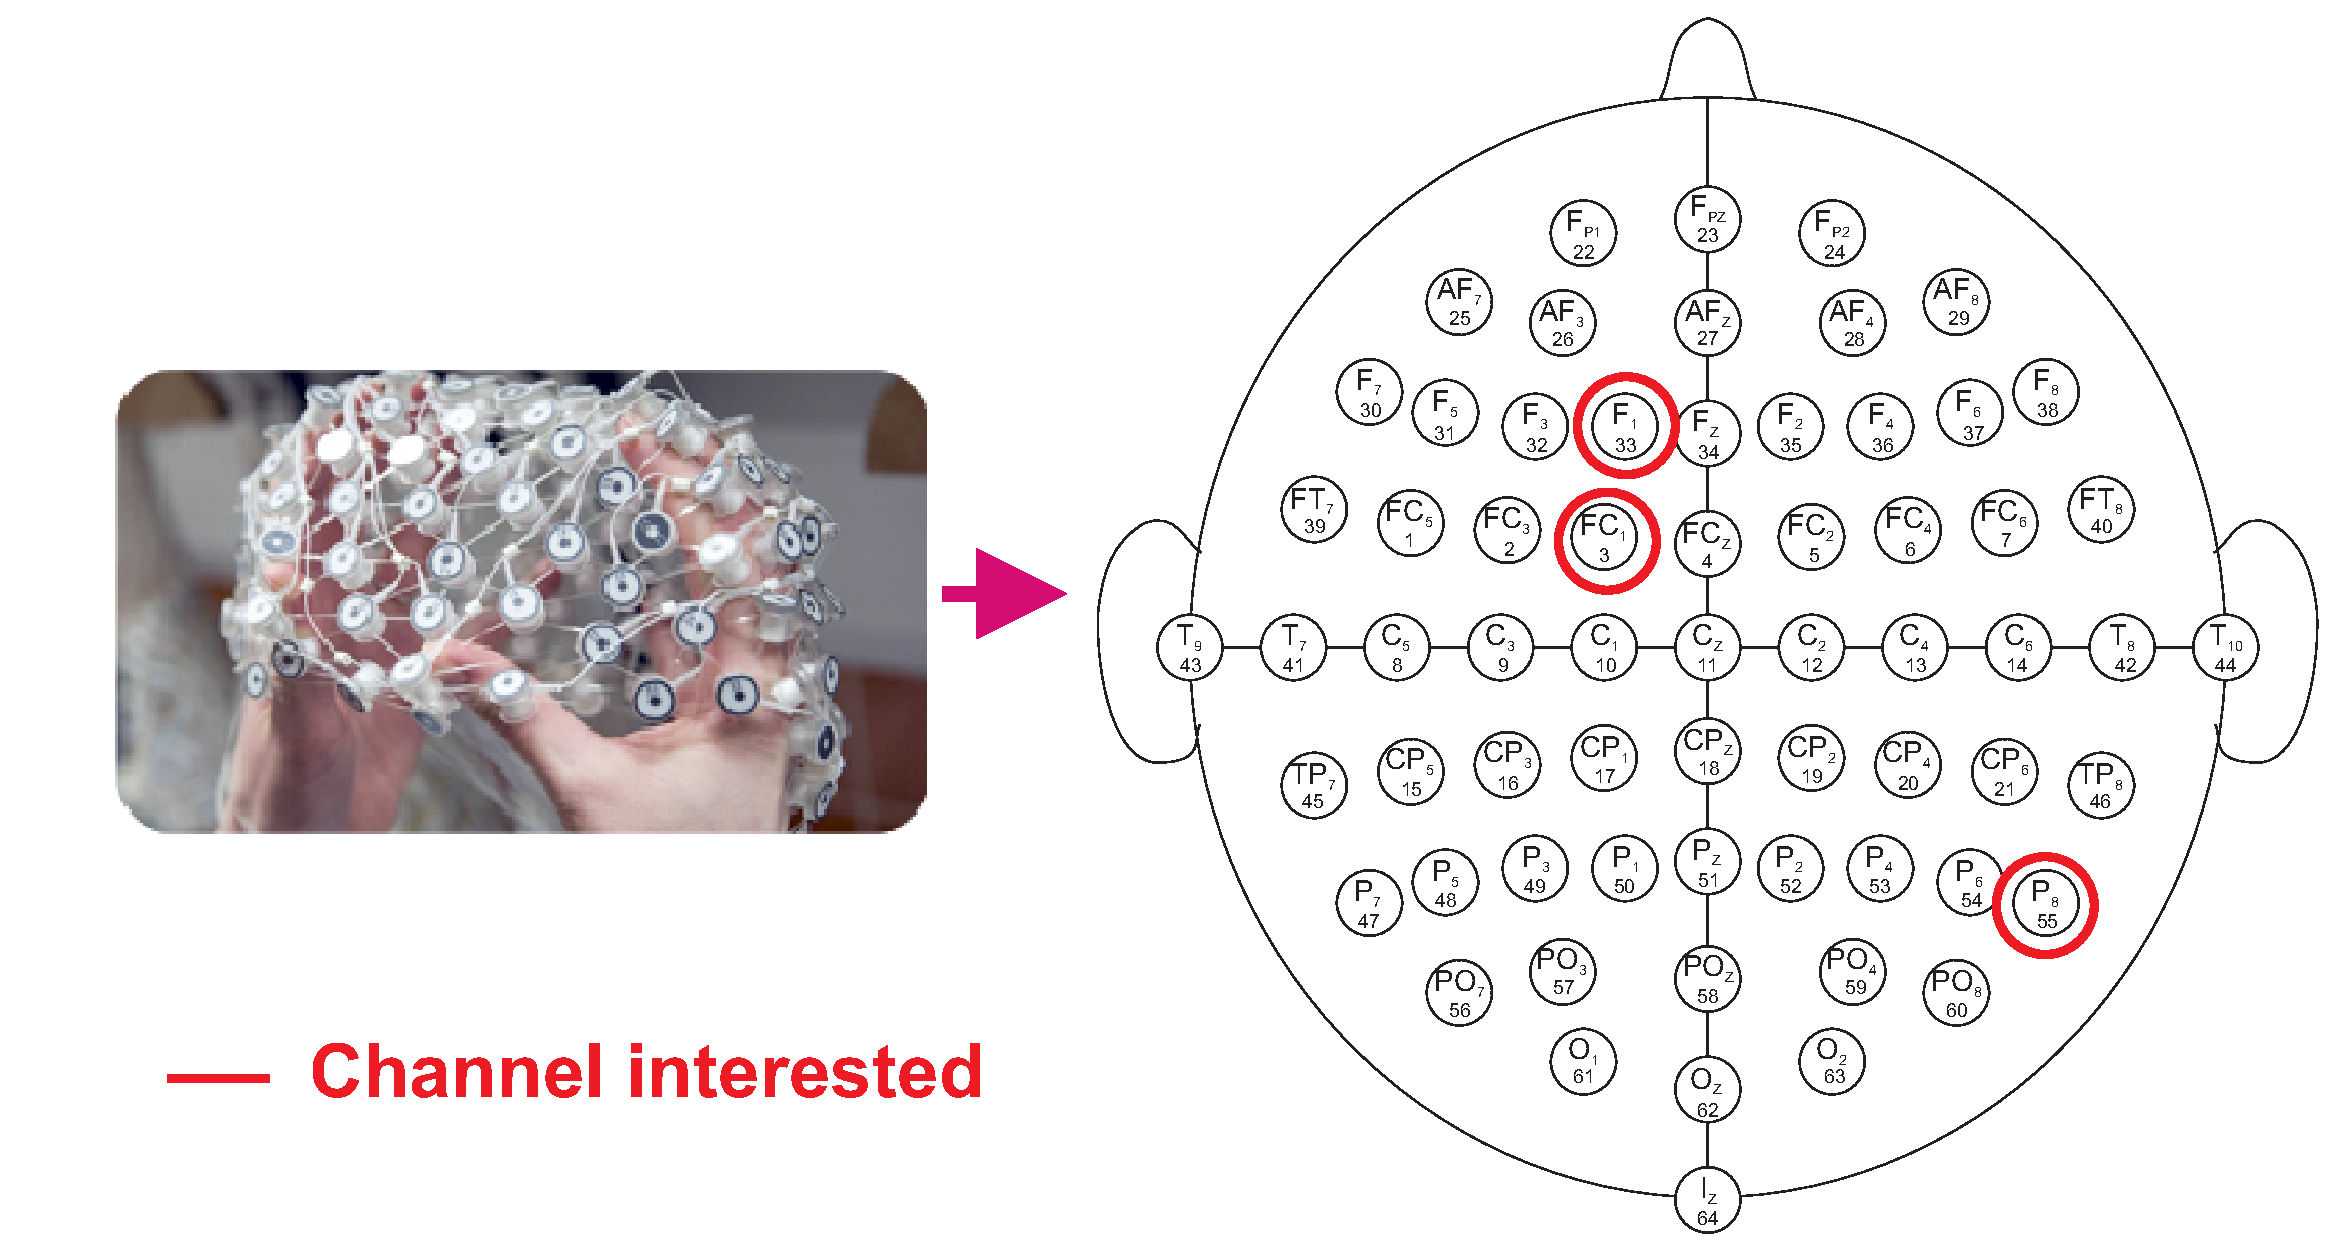
\includegraphics[width=0.9\columnwidth]{eeg.eps}
\vskip -3mm
\caption{\textbf{The 64-channel geodesic sensor distribution for measurement of EEG.}}\label{fig:eeg}
\vskip -5mm
\end{figure} 
 
To make the discussion more concrete and exemplify the mathematical formalism, we  investigated the statistical properties of a set of primary physiological processes (i.e, muscular, cardiac and neural processes). More specifically, we analyze the intramuscular EMG (iEMG), EEG and ECG signals from realistic clinical experiments. 
 
The iEMG signals are collected at different sites of the forearm muscles as shown in Figure~\ref{fig:emg}: (i) extensor digitorum (ED); (ii) flexor digitorum profundus (FDP); (iii) abductor pollicis longus (APL); (iv) flexor pollicis longus (FPL); (v) pronator teres (PT) and (vi) supinator (SUP), when the subject is asked to relax 6 seconds, then do the finger flexion at a consistent strength for 10 seconds. The ADInstruments data acquisition system sampled the iEMG at 4 KHz.

The EEG signals are recorded by a 64-channel electroencephalogram acquisition system shown in Figure~\ref{fig:eeg} that monitors the brain activity of 109 subjects when they are performing motor and imagery tasks upon noticing objects appearing on the screen~\cite{Physio_EEG}. Each subject is asked to open and close the corresponding fists or feet as a function of where the target appears. Each individual performed 14 experimental runs consisting of one minute with eyes open, one minute with eyes closed, and three two-minute runs of interacting with the target. The data set is collected by BCI2000 system with a sampling rate of 160Hz.
\begin{figure}%[htb]
\centering
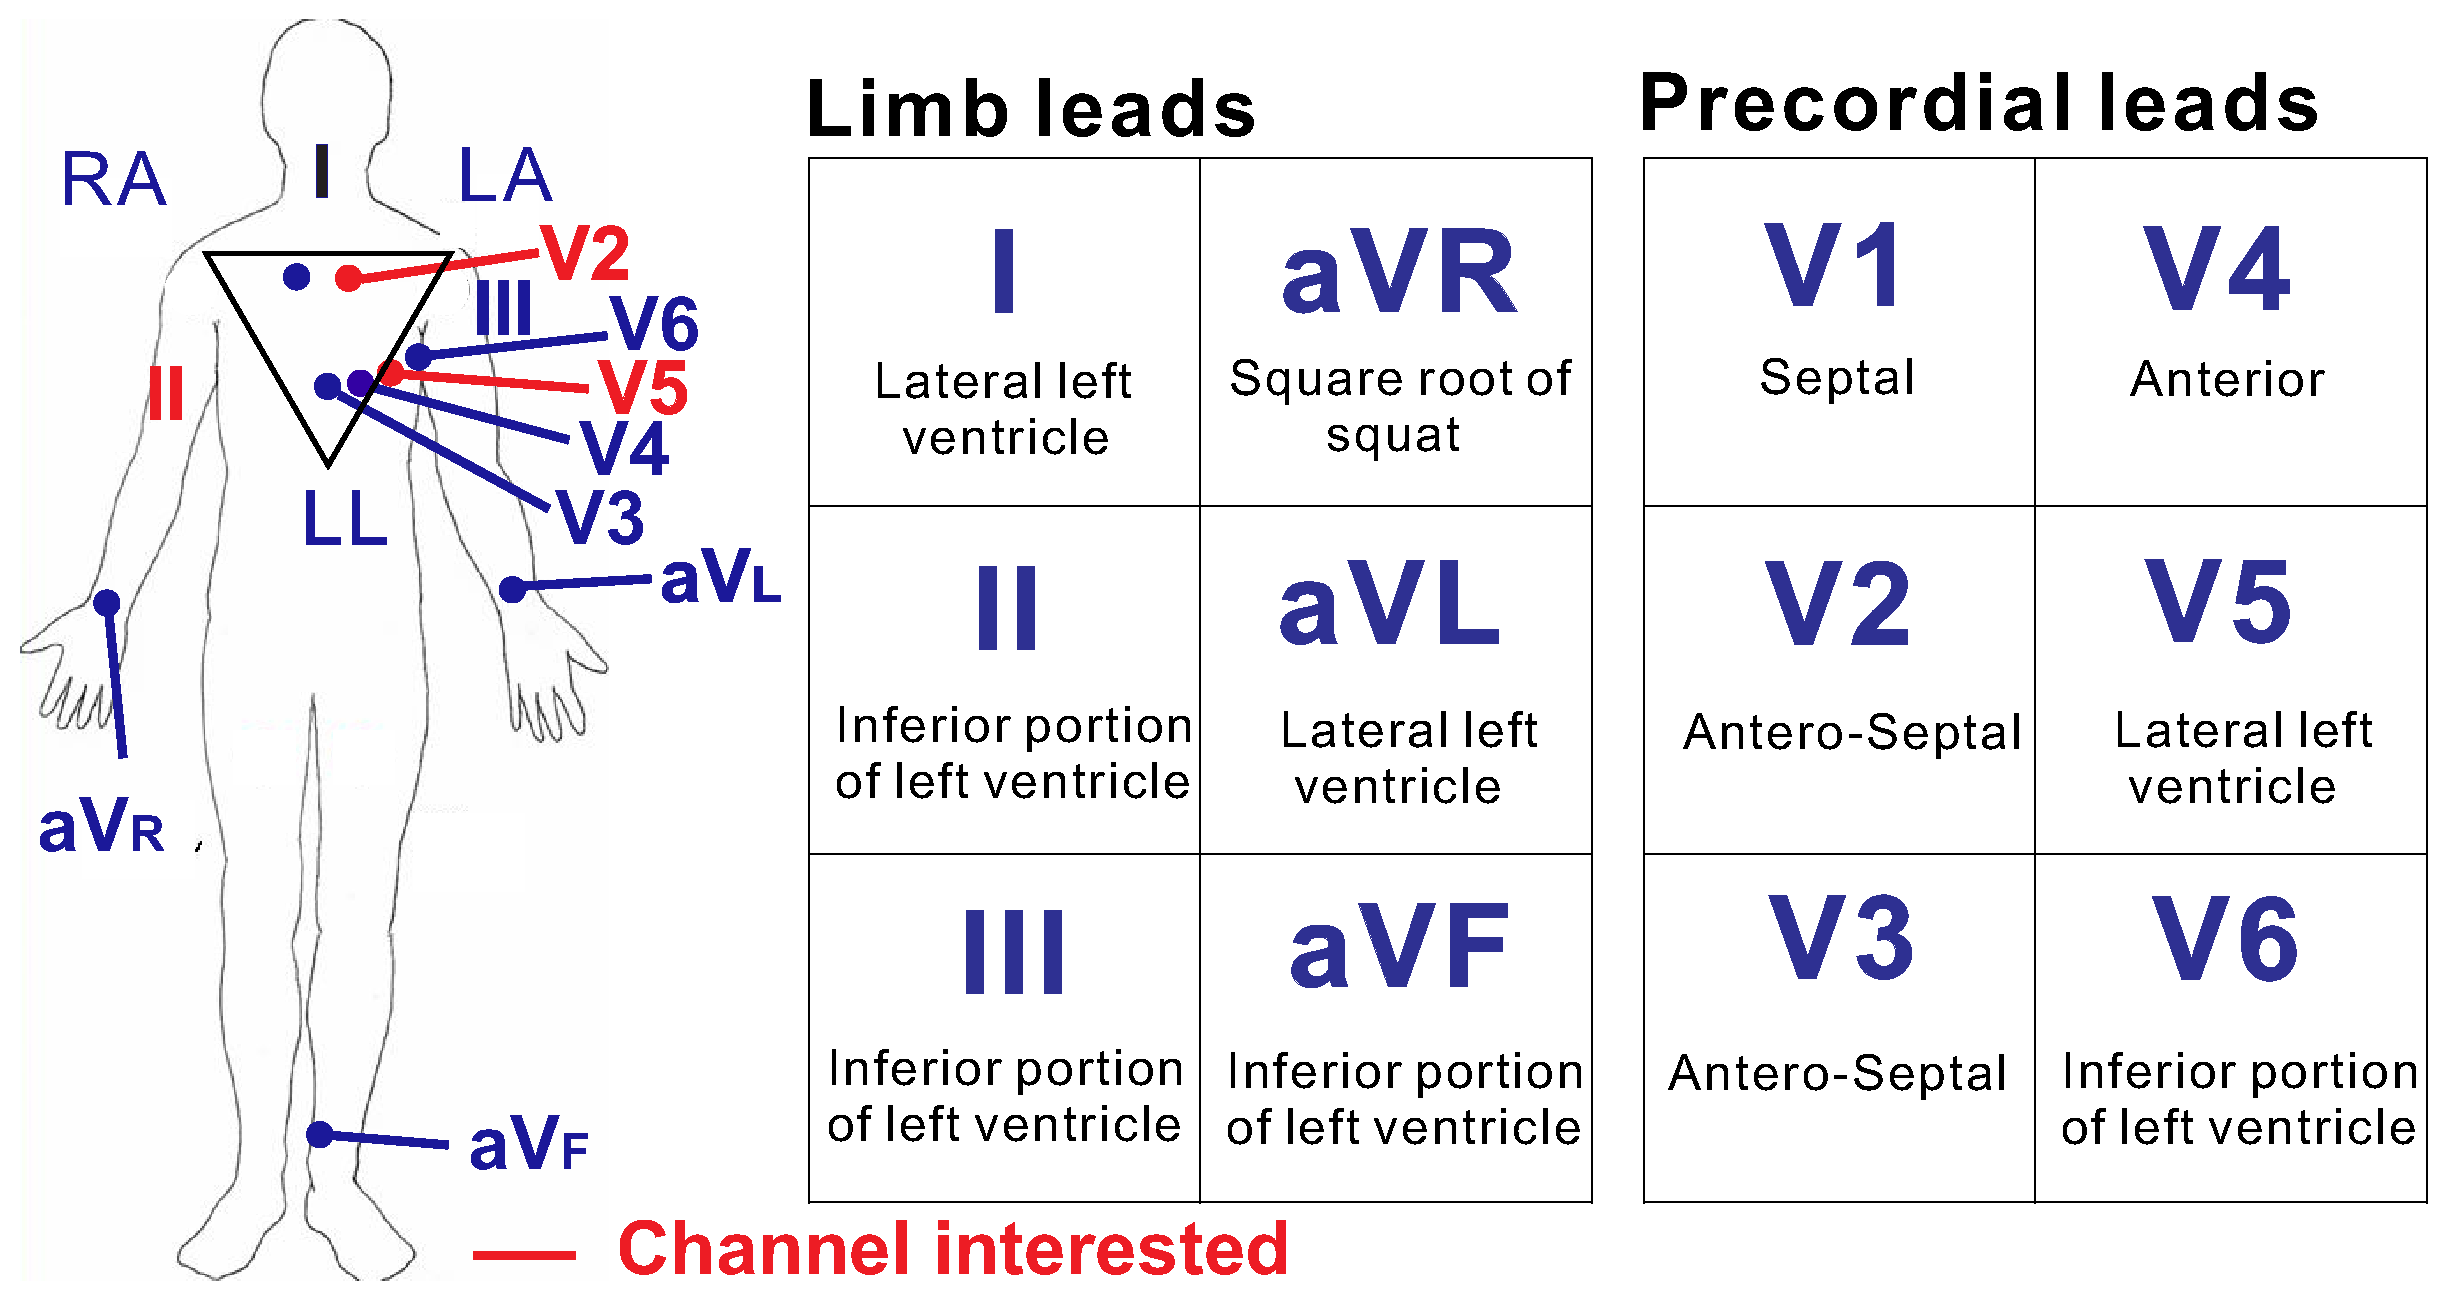
\includegraphics[width=0.9\columnwidth]{ecg.eps}
\caption{\textbf{The deployment of 12-lead ECG system used in the experiment is shown. }}\label{fig:ecg}
\vskip -6mm
\end{figure} 
The raw clinical ECG data was extracted from the PTB diagnostic ECG database~\cite{bousseljot1995nutzung}. Data on $52$ healthy subjects (13 women, age $48\pm 19$ and $39$ men, age $42\pm 14$) was obtained by the National Metrology Institute of Germany. Each subject’s record includes 15 different signals simultaneously acquired: the conventional 12-lead (I, II, III, aVR, aVL, aVF, V1, V2, V3, V4, V5, and V6) and 3 Frank orthogonal leads (VX, VY, and VZ) as shown in Figure~\ref{fig:ecg}. Each signal is digitalized at 1000Hz, with a signal bandwidth of 0Hz to 1KHz and with 1 uV LSB resolution. 
\subsection{Investigation of Non-Exponential System Dynamics}
\begin{figure}[!htb]
\centering
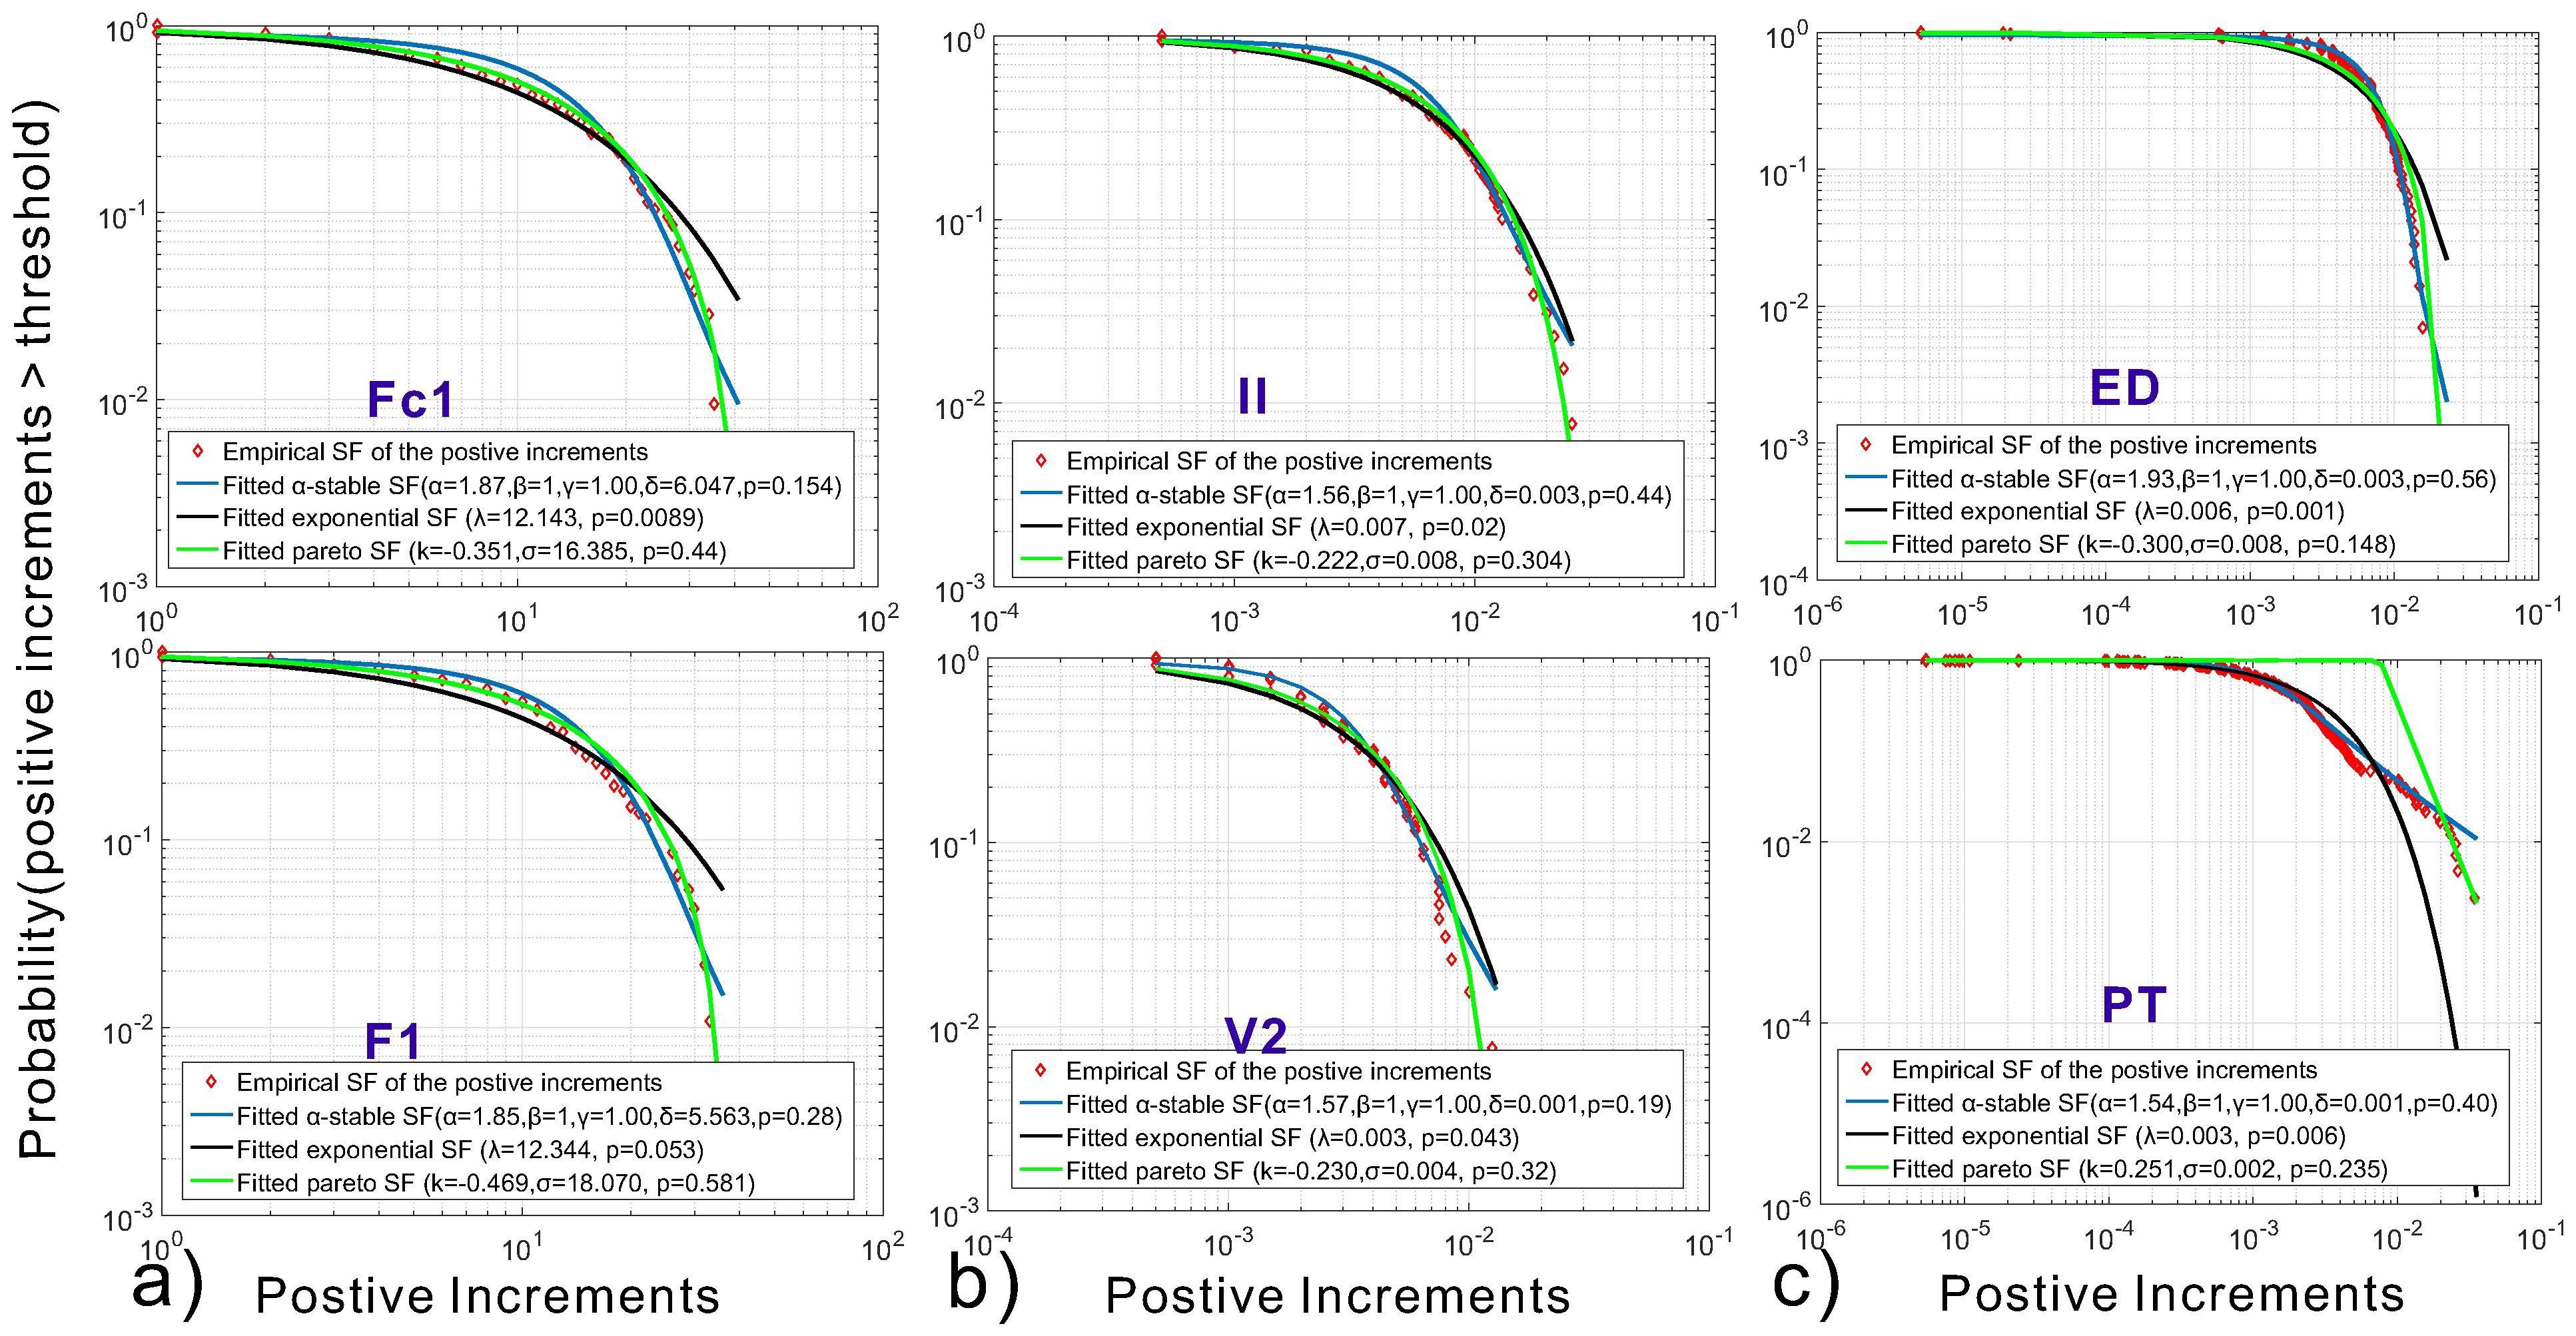
\includegraphics[width=1\columnwidth]{stats_overall_2.eps}
\vskip -3mm
\caption{\textbf{Empirical survival cumulative distribution functions and maximum likelihood best fitting $\alpha$-stable, exponential and Pareto distributions for magnitude increments in selected EEG, ECG and EMG channels. Figure (a)-(c) show the probabilities of the positive increments in magnitude exceeding a threshold value. P-value is obtained by performing a two-sample Kolmogorov-Smirnov test with the null hypothesis that the measurements come from the same distribution as the postulated $\alpha$-stable, exponential or Pareto distribution.}}\label{fig:stat_result}
\vskip -5mm
\end{figure}  

In the first set of experiments, we study the stochastic nature of magnitude increments (positive and negative) in all physiological processes considered to distinguish between exponential and power law behavior or between Gaussian and non-Gaussian cases. More specifically, we perform a statistical analysis to first estimate the empirical cumulative distribution function (CDF) and its support of the physiological process magnitude positive and the absolute value of negative increments. By fitting the measurements to the postulated stochastic models, we estimate the parameters of \textbf{i)} an $\alpha$-stable distribution, \textbf{ii)} exponential distribution and iii) Pareto distribution via maximum likelihood method. Then the CDFs of three stochastic models are generated based on the estimates of the model parameters.  

To quantify the statistical confidence of model fitting, we performed the two-sample Kolmogorov-Smirnov test between the measurements and the generated stochastic processes with identified $\alpha$-stable, exponential and Pareto distribution parameters. The null hypothesis assumes the measurements come from the same distribution as the postulated distributions with significance of 0.05. As a case study, we report the results of a selected set of physiological channels from the subjects that best illustrate their stochastic natures. Both positive and negative increments are studied and we visualize the experiments considering the positive increments in Figure~\ref{fig:stat_result}. Figure \ref{fig:stat_result}.(a-c) show how two models fit to the empirical survival function (SF) of a set of EEG (a), ECG (b) and iEMG (c) signal channels in the corresponding experiments, respectively. The interested channels are highlighted in Figure~\ref{fig:emg}-\ref{fig:ecg}. In all subfigures, the red squares correspond to the empirical SF, the blue lines, the black lines and the green lines represent the best-fitted $\alpha-$stable distribution, exponential distribution and Pareto distribution, respectively. The retrieved model parameters and p-values are reported in both the plot legends and Table \ref{tab:pos_neg}. 

By examining the figures, we can make several important observations: i) The null hypothesis that the positive increments follow an exponential distribution is rejected in all physiological channels we considered with p-value ranging from $0.001$ to $0.043$. This suggests that magnitude variation over time domain strongly contradicts with an exponential law which is a well-adopted assumption in previous work. 

ii) The p-value well coincides with our visual inspection that the exponential SF fitting (black lines) deviates the empirical SF in all the channels considered. Instead, the Pareto distribution and the $\alpha$-stable fitting better represent the stochastic properties of the signal variations over time in all channels. This suggests the existence of fractality which is governed by a power-law distribution as postulated by equation~(\ref{multidimensionalTP}), which also coincides with our following observation.

 iii) For all channels that can be better characterized by an $\alpha$-stable distribution or Pareto distribution, the estimated stability parameters $\alpha$ are all smaller than 2 where $\alpha=2$ corresponds to a Gaussian process. For $\alpha < 2$, stable distributions have one tail (when $\alpha < 1$ and $\beta = \pm 1$) or both tails (all other cases) that are asymptotically \textit{power laws} with heavy tails. This is best illustrated in FDP and PT channel of iEMG signals where the empirical distribution fits well to the $\alpha-$stable distribution up to a certain transition point where the empirical SF starts to obey the Pareto distribution (i.e., power-law). This suggests the existence of fractality in these physiological processes which is aligned with our analytical prediction made by Theorem 1, hence justifying the application of the proposed fractal dynamical state equation described in equation~(\ref{vectorARFIMA1}). The similar conclusion can also be reached by investigating the stochastic properties of the negative increments (see Table~\ref{tab:pos_neg}) in physiological processes.
\subsection{Efficacy Evaluation of FDSE for Physiological Processes}
\begin{figure}%[!htb]
\centering
\includegraphics[width=1\columnwidth]{overall_2.eps}
\vskip -5mm
\caption{\textbf{Fitting the model to physiological measurements of EEG, ECG and iEMG considering i) FDSE with no coupling matrix $A$, ii) FDSE with coupling matrix $A$ and iii) Vector ARMA model with no fractal exponents.}}\label{fig:exp_result}
\vskip -4mm
\end{figure}  

\begin{table}[ht]
\caption{KS-test and ML best-fitting parameters of $\alpha$-stable, exponential and Pareto distributions for selected channels}
\vskip -4mm
\begin{center}
\scalebox{0.72}{
\begin{tabular}{|c|c|c|c|c|c|c|c|c|c|c|c|c|c|c|c|}
    \hline
    \multirow{2}{*}{Channel}&\multicolumn{6}{c|}{Positive increments} & \multicolumn{6}{c|}{Negative increments} \\
    \cline{2-13}
    &$\alpha$,$\beta$,$\gamma$,$\delta$&$p_{stbl}$&$\lambda$&$p_{exp}$&k,$\sigma$&$p_{par}$&$\alpha$,$\beta$,$\gamma$,$\delta$&$p_{stbl}$&$\lambda$&$p_{exp}$&k,$\sigma$&$p_{par}$\\
    \hline
    Fc1&1.87,1,1,6.05&0.15& 12.14& 0.0089& -0.35,16.39& 0.44 &1.56,1,1,5.56& 0.08& 14.47& 0.071& 0.39, 20.04& 0.18\\
    \hline
    F1& 1.85,1,1,5.56 &0.28& 12.34& 0.053& -0.47,18.07& 0.58& 1.89,1,1,6.02 & 0.15& 11.29& 0.05& -0.43,16.18& 0.73\\
    \hline
    P8& 1.57,1,1,4.62& 0.19& 11.38& 0.0025& -0.19, 13.56& 0.16& 1.88,1,1,6.17& 0.01& 11.2& 0.03& -0.25,14.03& 0.16\\
    \hline
    II& 1.56,1,1,0.003& 0.44& 0.007& 0.02& -0.22, 0.008& 0.30& 1.69,1,1,0.003& 0.24& 0.006& 0.0089& -0.20, 0.007& 0.21\\
    \hline
    V2& 1.57,1,1,0.001& 0.19& 0.003& 0.043& -0.23,0.004& 0.32& 1.8,1,1,0.002& 0.05& 0.004& 0.01& -0.40,0.005& 0.38\\
    \hline
    V5& 1.4,1,1,0.001& 0.15& 0.003& 0.0017& -0.19,0.004& 0.33& 1.93,1,1,0.002& 0.01& 0.003& 0.047& -0.42,0.005& 0.49\\
    \hline
    ED& 1.93,1,1,0.003& 0.56& 0.006& 0.001& -0.30,0.008& 0.15& 1.92,1,1,0.003& 0.1& 0.005& 0.034& -0.29,0.007& 0.65 \\
    \hline
    FDP& 1.09,1,0.59,0.004& 0.36& 0.014& 0.01& 0.18,0.011& 0.22 &0.49,1,1,0.003& 0.15& 0.021& 0.0001& 0.87,0.007& 0.47\\
    \hline
    PT& 1.54,1,1,0.001& 0.4& 0.003& 0.006& 0.25,0.002& 0.24& 1.41,1,1,0.001& 0.37& 0.002& 0.004& 0.051,0.002& 0.68\\
    \hline
\end{tabular}}
\end{center}
\label{tab:pos_neg}
\vskip -5mm
\end{table}
The investigation of the stochastic characteristics of the processes considered verified the existence of non-Gaussian and fractality (non-linearity) in the physiological systems. Therefore, the dynamical behaviors of these systems in time and spatial domain can not be accurately described by the conventional methods that assumes a stationary and Markovian system state equation with short-term memory. In what follows, we present the second set of experiments where we are interested in the spatial (i.e, interdependency across multiple channels) and temporal (i.e., how previous system state passes down its influence to current system dynamics) dependency structure of the physiological processes. We evaluated the capability of the proposed FDSE in capturing the complex dynamical behaviors of physiological processes. More precisely, we employed a least-square error estimator proposed in~\cite{xue2016spatio,xue2016minimum} to identify the model described by equation (\ref{vectorARFIMA1}). After the identification of the model, we evaluate the model adequacy by comparing the physiological measurements and predicted model output as goodness-of-fit metrics. 

To compare with the Vector ARMA (VARMA) model and understand the significance of coupling the fractal exponents into FDSE (i.e., considering the long term memory in system state dynamics), we report three experimental settings: i) only fractal exponents $\beta$ are considered (i.e., assuming an identify matrix for $A$ in equation (\ref{vectorARFIMA1})); ii) only coupling matrix $A$ is considered (i.e., assuming $\beta_{i}=1$ which reduces to VARMA type model) and iii) both coupling matrix and fractal exponents $\beta$ are considered (i.e., FDSE). We show the comparison results of a selected set of channels from EEG (a), ECG (b) and iEMG (c) measurements in Figure~\ref{fig:exp_result}, respectively. The blue lines show the actual measurements. The orange lines represent the predicted model output where only fractal exponents are considered (i.e, setting i). The yellow lines and the magenta lines correspond to setting ii and iii, respectively. We use the system identification approach proposed in \cite{xue2016spatio}. The estimated fractal exponents range from $ 0.30$ to $0.66$, $0.94$ to $1.19$ and $0.18$ to $0.61$ for EEG, ECG and iEMG signals, respectively, hence verifying the existence of fractality.

 Two key observations can be made for Figure~\ref{fig:exp_result}: i) In all experiments we considered, the efficacy of incorporating the fractal exponents that captures the long-term memory effect in system dynamics can be best illustrated by the comparison between the predicted model output and actual measurements. In spite of the difference in magnitude, the predicted model output stays close to the actual measurement in terms of preserving critical system state transition behaviors. Intuitively, the predicted model output preserves turning points and the envelope of the state dynamics of actual physiological processes. This is primarily important for construction of a time-series model capable of characterizing the physiological processes. Vital changes in bio-markers of the physiological system usually correspond to \textit{infrequent anomalies} (e.g., the abrupt decrease/increase in blood glucose/blood pressure or excessive brain activity caused by epilepsy). The failure of the model in capturing such vital changes translates to false negative errors and might lead to irreversible undesired consequences. In contrast, the fitted VARMA models without considering the long-term memory have the tendency to smooth away the sudden changes in model output in order to minimize least-square errors as a consequence of the regression process.
 
 ii) Comparing the goodness-of-fit between FDSE models with and without considering coupling matrix $A$ that encodes the interdependency across different channels leads to interesting findings. As shown in the figure, the FDSE without matrix considering $A$ tends to overestimates the signal magnitude as a result of accumulating the influence of the previous system states over a long time course. In contrast, FDSE model with coupling matrix $A$ in all experiments aligns well with the actual measurements suggesting its adequacy in characterizing the physiological processes. The performance difference can be understood as follows: the FDSE assuming an identity matrix $A$ has no knowledge of how coupled physiological processes contribute to the state transition dynamics of each other. As a result, given a specific channel, the estimation process tries to compensate the contribution from other channels by assuming a long lasting influence from the previous system states. By incorporating the matrix $A$, the predicted model output is well regulated to adequately fit to actual measurements by coupling the interdependency between different channels of the physiological signals.
\section{Summary}
\label{Conclusion}
Understanding the implications of the degree of nonlinearity and the nature of fractality (i.e., distinguishing between fractality in the magnitude increments (space) of one variable with respect to other variables and the fractality in the inter-event times) represents the motivation of this work. We generalize the linear / nonlinear dynamic causal approaches, by adopting a statistical physics inspired probabilistic description of various processes representing the evolution of a complex system and incorporating the statistics of the magnitude increments and the inter-event times into the mathematical expression of the master equation. 

First, this new approach allows to capture the power law and nonlinear interactions that exist between the magnitude increments and the inter-event times of one stochastic process on one hand, and the inter-dependencies between the magnitude increments and the inter-event times of one process and other processes, on the other hand. Second, it provides a mathematical strategy for modeling of complex systems whose dynamics exhibits a mixture of Markovian and non-Markovian evolution. Relying on conditional probabilistic description on how ordered sequence of magnitude increments and the inter-event times affect the overall system dynamics allows to define new multivariate causal inference techniques that take into account the non-Markovian nature of the dynamics. This is left for future work. Moreover, it allows to mathematically justify the adoption of a class of mathematical model that could potentially complement current Bayesian model selection strategies. The presented mathematical framework could be enriched by combining it with other techniques from statistical machine learning and signal processing for developing new modeling strategies for complex interdependent networks. Third, the proposed causal modeling of complex dynamics can be integrated as the core of the cognizant cyber-physical systems in a widely ranged CPS applications to be able to understand, describe, predict and control the underlying physical processes.

